\section{Spezifikation der Anwendung}\label{specification} \thispagestyle{nomarkstyle}
In diesem Kapitel werden die Anforderungen an das System und die daraus resultierenden Anwendungsfälle beschrieben.
Anschließend wird eine System-Abgrenzung vorgenommen, sowie auf die inhaltliche Gestaltung der Anwendung eingegangen.

\subsection{Anforderungen}
Die Kernanforderung an das System ist es, dem Benutzer zu ermöglichen, sich Artikel anzuschauen und diese bestellen zu können.
Darüberhinaus soll es einem Administrator möglich sein, neue Artikel anzulegen oder bestehende zu löschen.
Dafür ist die Implementierung eines Rollensystems nötig, um die Benutzergruppen unterscheiden zu können.

Für die Bestellung von Artikeln ist es nötig, dass sich ein Benutzer in der Anwendung registrieren und seine persönlichen Daten angeben kann.
Um eine Bestellung aufzugeben muss sich der registrierte Benutzer am System anmelden können.
Die detaillierte Beschreibung der für diese Funktionalitäten benötigten Anwendungsfälle findet sich in \cref{usecases}.
\subsection{Nichtfunktionale Anforderungen}
Die Anwendung sollte von allen gängigen Browsern in neueren Versionen sowie auf mobilen Geräten darstellbar sein.
Sensible Daten, wie die persönlichen Daten der Anwender, müssen vor unbefugtem Zugriff geschützt sein.
Der Admin-Bereich sollte getrennt vom Webshop sein.

Im Fehlerfall soll der Benutzer über Hinweise darauf aufmerksam gemacht werden.
Dabei sollen interne Fehlermeldungen des Servers, sowie unverständliche Fehlercodes vor dem Anwender verborgen werden.
Um die Benutzerfreundlichkeit der Anwendung zu sichern, sollte sich die Antwortzeit des Servers in einem vertretbaren Rahmen bewegen (Richtwert 3 Sekunden).
\subsection{Hauptanwendungsfälle}\label{usecases}
Das folgende Diagramm zeigt die Anwendungsfälle für den Benutzer und Administrator, sowie die jeweils beteiligten System-Komponenten.
Die Anwendungsfälle werden im Anschluss im Einzelnen betrachtet.
\begin{figure}[ht!]
	\centering
	\includegraphics[width=\linewidth]{bilder/kap4/use_cases}
	\caption{Anwendungsfalldiagramm mit den Hauptanwendungsfällen}
	\label{fig:usecases}
\end{figure}

\subsubsection{Benutzer- bzw. Kunden-Anwendungsfälle}
\paragraph{Register (Registrierung)}$\;$ \\
Ein Benutzer soll sich durch Angabe seiner persönlichen Daten beim System registrieren können.
Die dafür nötigen Pflichtangaben sind:
\begin{itemize}
\item Anrede
\item Vorname
\item Nachname
\item Geburtsdatum
\item E-Mail-Adresse
\item Passwort
\item Straße und Hausnummer
\item Stadt
\item Postleitzahl
\item Land
\end{itemize}
Zusätzlich soll es bei der Registrierung möglich sein, eine abweichende Lieferadresse einzugeben.
Nach der Registrierung muss es dem Benutzer möglich sein, sich am System anzumelden.
Um Artikel anschauen zu können, muss ein Besucher der Seite nicht registriert oder angemeldet sein.

\paragraph{Login/Logout}$\;$ \\
Registrierte Nutzer können sich durch die Eingabe ihrer E-Mail-Adresse und ihrem Passwort im Shop einloggen.
Bei einer fehlerhaften Eingabe soll eine Meldung ausgegeben werden.
Zudem soll die Login-Seite neuen Benutzern die Möglichkeit bieten, sich zu registrieren.
Der Login ist Voraussetzung für folgende weitere Use Cases: Anzeigen/Bearbeiten der persönlichen Informationen, Zum Warenkorb hinzufügen, Bestellung aufgeben und Bestellhistorie einsehen.
Außerdem muss beim Einloggen auch der Warenkorb des jeweiligen Benutzers geladen werden, da dieser Artikel enthalten kann, die der User beim letzten Besuch des Shops hineingelegt hat.
Beim Logout wird der Benutzer wieder abgemledet und kann ohne einen erneuten Login nicht mehr auf seine Daten zugreifen oder die benutzerspezifischen Anwendungsfälle ausführen.

\paragraph{Show/edit user details (Anzeigen/Bearbeiten der persönlichen Informationen)}$\;$ \\
Einem eingeloggten Benutzer soll es möglich sein, seine persönlichen Daten einzusehen und zu ändern.
Dafür soll ihm eine übersichtliche Seite mit allen Informationen und Funktionalitäten zur Verfügung stehen.
Folgende Änderungen sollen möglich sein:
\begin{itemize}
\item Adressdaten (Liefer- und Rechnungsadresse)
\item E-Mail-Adresse
\item Passwort
\end{itemize}
Für eine Passwort-Änderung muss auch das bisherige Passwort eingegeben werden.

\paragraph{Show shopping cart (Warenkorb anzeigen)}$\;$ \\
Der Warenkorb soll jederzeit über einen Button am oberen Rand der Seite erreichbar sein.
Ist der Benutzer noch nicht angemeldet, soll er beim Klick auf den Warenkorb auf die Login-Seite umgeleitet werden.
Über einen Klick auf den Button wird eine detaillierte Auflistung der Artikel, die dem Warenkorb hinzugefügt wurden, sowie der Gesamtwert des Warenkorbs angezeigt.
In der Detailansicht soll auch eine Anpassung der Menge für jeden Artikel und das Entfernen eines Artikels aus dem Warenkorb möglich sein.
Der Warenkorb soll gespeichert werden, so dass der Einkauf zu einem späteren Zeitpunkt fortgesetzt werden kann.
\paragraph{Add to shopping cart (Zum Warenkorb hinzufügen)}$\;$ \\
Artikel sollen jederzeit zum Warenkorb hinzugefügt werden können, wenn ein Benutzer eigeloggt ist. Sowohl in einer Übersicht über mehrere Artikel als auch in der Detailansicht eines Artikels soll dies möglich sein.
Das Hinzufügen eines Artikels zum Warenkorb soll dem Benutzer rückgemeldet werden, damit er erkennt, dass die Aktion erfolgreich war.
\paragraph{Place order (Bestellung aufgeben)}$\;$ \\
Über die Detailansicht des Warenkorbs sollen Bestellungen aufgegeben werden können.
Vor der tatsächlichen Auslösung der Bestellung soll dem Benutzer eine Zusammenfassung gezeigt werden, die neben den einzelnen Artikeln auch seine Adressdaten und den Gesamtwert der Bestellung enthält.
In dieser Übersicht soll auch die Menge für die einzelnen Artikel angepasst werden können.
Nach der Bestätigung durch den Nutzer soll die Bestellung ausgelöst und eine entsprechende Meldung ausgegeben werden.
\paragraph{Show order history (Bestellhistorie einsehen)}$\;$ \\
Sämtliche getätigte Bestellungen sollen dem Benutzer jederzeit einsehbar sein.
Dafür soll eine Liste mit den Bestellungen aufgeführt werden, für die über einen Button am Ende der Zeile die Details der jeweiligen Bestellung eingesehen werden können.
\paragraph{Search products (Artikelsuche)}$\;$ \\
Die Suche nach Artikeln im Shop soll über eine hierarchische Unterteilung in Kategorien realisiert werden.
Unter den Hauptkategorien kann der Benutzer in Unterkategorien auswählen, wonach er suchen möchte.
Dadurch kann erreicht werden, dass ein Nutzer seinen Wunsch so weit präzisieren kann, dass er nur noch eine überschaubare Menge an Artikeln gezeigt bekommt, die seinen Kriterien entsprechen.
\paragraph{Filter products (Artikel filtern)}$\;$ \\
Um die Suche nach Artikeln weiter zu unterstützen, soll eine Filterung möglich sein, die eine Auswahl nach verschiedenen Artikelmerkmalen bietet.
So soll der Benutzer beispielsweise nach der Marke oder der Farbe filtern können, um nur Produkte dieser Marke oder Farbe angezeigt zu bekommen.
\paragraph{Show product details (Detailansicht eines Artikels)}$\;$ \\
Durch einen Klick auf den Namen oder das Vorschaubild eines Artikels, soll dessen Detailansicht erscheinen, die alle verfügbaren Informationen zu diesem Artikel zeigt.
\subsubsection{Administrator-Anwendungsfälle}
Anwendungsfälle für Administratoren sind nur für Benutzer zugänglich, die über die entsprechende Rolle verfügen.
Der Bereich für alle derartigen Operationen soll getrennt vom restlichen Shop sein und ist vor unbefugtem Zugriff zu schützen.
\paragraph{Login/Logout}$\;$ \\
Die Anmeldung für Administratoren soll über eine gesonderte URL erfolgen, die nicht im Shop verlinkt ist.
Sie erfolgt ebenfalls über die E-Mail-Adresse und ein Passwort. Zusätzlich muss geprüft werden, ob der Benutzer über Administrator-Rechte verfügt.
Erst nach erfolgreicher Authentifizierung und Verifikation der Rolle sollen die anderen Funktionen erreicht werden können.
\paragraph{Create new Admin (Neuen Admin hinzufügen)}$\;$ \\
Die Rolle des Admin kann nur von einem bestehenden Admin vergeben werden.
Voraussetzung ist ein bestehendes Nutzerkonto (Anmeldung beim Shop) für den Benutzer, der künftig Administrator sein soll.
Über eine Liste mit allen registrierten Nutzern, soll ausgewählt werden können, welcher Benutzer zu einem Admin gemacht werden soll.
In gleicher Weise kann einem bestehenden Admin auch seine Rolle entzogen werden.
\paragraph{Add/edit product (Artikel hinzufügen/ändern)}$\;$ \\
Um neue Artikel für den Shop anzulegen oder bestehende zu ändern/löschen, soll es jedem Admin möglich sein, über eine Eingabemaske entsprechende Angaben zu machen.
Für das Anlegen neuer Artikel muss das Hochladen von Bilddateien ermöglicht werden.
Neue Artikel oder Änderungen sollten sofort im Shop integriert werden.
\subsection{System-Abgrenzung}
Das System beschränkt sich auf einen Web-Server mit der Anwendung, die in Shop und Admin-Bereich unterteilt ist und der Datenbank.
\begin{figure}[ht!]
	\centering
	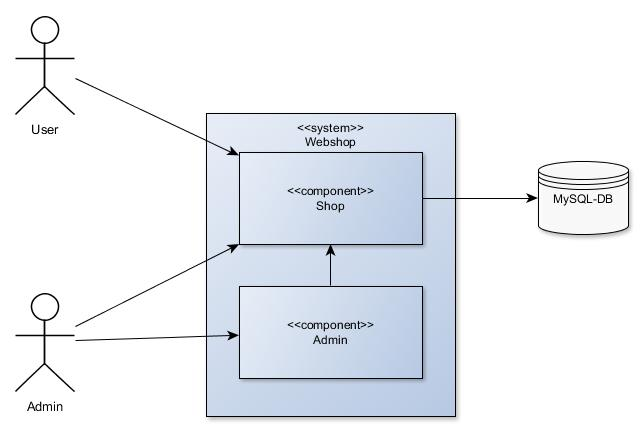
\includegraphics[width=\linewidth]{bilder/kap4/system_abgrenzung}
	\caption{Systemkontext}
	\label{fig:system_context}
\end{figure}
\cref{fig:system_context} zeigt den System-Kontext der Anwendung.
\subsection{Inhaltliche Definition}
Für den thematischen Inhalt des Webshops wurde das Thema Wolle und Handarbeit gewählt.
Der Fokus liegt dabei auf der Wolle. Als Hauptkategorien wurden Wolle, Stricken, Häkeln, Zubehör und Bücher festgelegt.
Um das Thema auch in der Gestaltung zu spiegeln, wurde viel Wert auf eine freundliche, ansprechende Oberfläche gelegt.

